\documentclass{article}

%% Page Margins %%
\usepackage{geometry}
\geometry{
    top = 0.75in,
    bottom = 0.75in,
    right = 0.75in,
    left = 0.75in,
}

\usepackage{amsmath}
\usepackage{graphicx}
\usepackage{parskip}

\title{Lab 5: Counters and Clocks}

% TODO: Enter your name
\author{Your Name}

\begin{document}
\maketitle

\section{Part I}

\begin{enumerate}
\item Export the subcircuit schematic as an image and include it in your report.

\begin{figure}[ht!]
    \centering
    % \includegraphics[width=0.65\textwidth]{lab5_counter2.png}
    \caption{A schematic of counter2.}
    \label{f:counter2}
\end{figure}

\item Export the subcircuit schematic as an image and include it in your report.

\begin{figure}[ht!]
    \centering
    % \includegraphics[width=0.65\textwidth]{lab5_counter4.png}
    \caption{A schematic of counter4.}
    \label{f:counter4}
\end{figure}

\item Export the timing diagram as an image and include it in your report.

\begin{figure}[ht!]
    \centering
    % \includegraphics[width=0.65\textwidth]{lab5_timing_counter4.png}
    \caption{A timing simulation of counter4.}
    \label{f:counter4_timing}
\end{figure}

\item Export the subcircuit schematic as an image and include it in your report.

\begin{figure}[ht!]
    \centering
    % 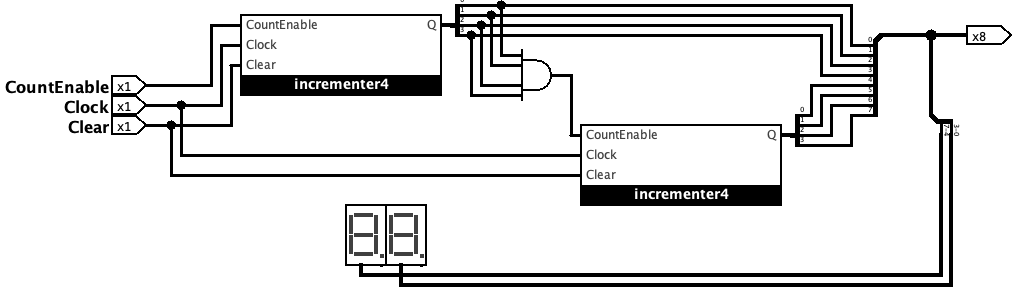
\includegraphics[width=0.65\textwidth]{lab5_counter8.png}
    \caption{A schematic of counter8.}
    \label{f:counter8}
\end{figure}

\end{enumerate}

\section{Part II}

\begin{enumerate}
\item Export the subcircuit schematic as an image and include it in your report.

\begin{figure}[ht!]
    \centering
    % 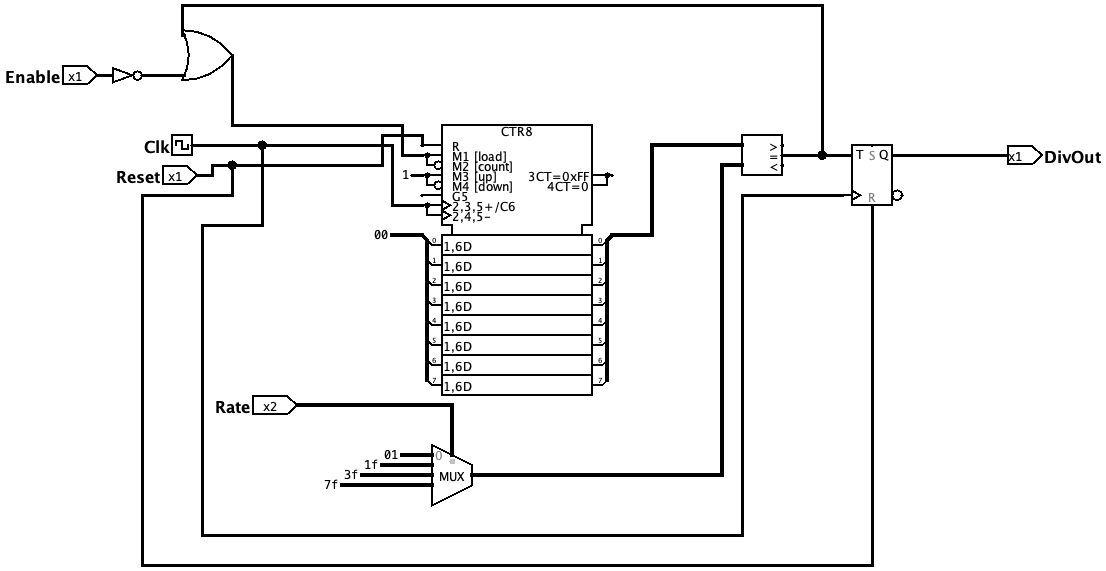
\includegraphics[width=0.65\textwidth]{lab5_rate_divider.png}
    \caption{A schematic of rate\_divider.}
    \label{f:rate_divider}
\end{figure}

\item Export the timing diagram as an image and include it in your report.

\begin{figure}[ht!]
    \centering
    % 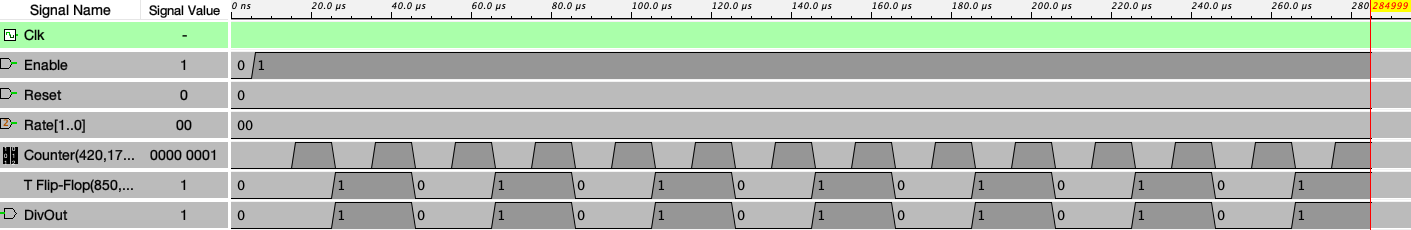
\includegraphics[width=0.65\textwidth]{lab5_timing_rate_divider.png}
    \caption{A timing simulation of rate\_divider.}
    \label{f:rate_divider_timing}
\end{figure}
\end{enumerate}

\section{Part III}

\begin{enumerate}
\item Fill in a table with your binary representation of each letter from S to Z.

\begin{table}[ht!]
\centering
\begin{tabular}{|c|l|c|} \hline
    \textbf{Letter} & \textbf{Morse Code} & \textbf{Pattern Representation (pattern length is \underline{\hspace{1cm}} bits)} \\ \hline

    S & \textbf{$\bullet$ $\bullet$ $\bullet$} & \hspace{2cm} \\ \hline
    T & \textbf{---} & \\ \hline
    U & \textbf{$\bullet$ $\bullet$ --- } & \\ \hline
    V & \textbf{$\bullet$ $\bullet$ $\bullet$ --- } & \\ \hline
    W & \textbf{$\bullet$ --- ---} & \\ \hline
    X & \textbf{--- $\bullet$ $\bullet$ ---} & 111010101110\\ \hline
    Y & \textbf{--- $\bullet$ --- ---} & \\ \hline
    Z & \textbf{--- --- $\bullet$ $\bullet$} & \\ \hline

\end{tabular}
\caption{Morse Pattern Representation with fixed bit-width}
\label{tab:morse:pattern}
\end{table}

\item Export the subcircuit schematic as an image and include it in your report.

\begin{figure}[ht!]
    \centering
    % 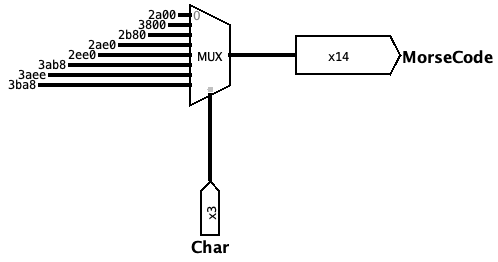
\includegraphics[width=0.65\textwidth]{lab5_morse_lut.png}
    \caption{A schematic of MORSE\_LUT.}
    \label{f:morse_lut}
\end{figure}
\end{enumerate}

\end{document}